\documentclass{beamer}

\usepackage[utf8]{inputenc}
\usepackage[brazil]{babel}
\usepackage{graphicx,hyperref,icmc,url}
\usepackage{subcaption}
\usepackage{multirow}

% The title of the presentation:
%  - first a short version which is visible at the bottom of each slide;
%  - second the full title shown on the title slide;
\title[Reconstrução de curvas por características robustas extraídas de imagens]{Reconstrução de curvas por meio de características robustas extraídas de imagens}

% Optional: a subtitle to be dispalyed on the title slide
\subtitle{}

% The author(s) of the presentation:
%  - again first a short version to be displayed at the bottom;
%  - next the full list of authors, which may include contact information;
\author[André Luís Mendes Fakhoury]{
    \Large{André Luís Mendes Fakhoury} \\ \medskip
    \small{NUSP: 4482145} \\
    \small{\href{mailto:andrefakhoury@usp.br}{\nolinkurl{andrefakhoury@usp.br}}} \\ \bigskip
    \small{Orientador: João do Espirito Santo Batista Neto} \\ \bigskip
    \large{Vinculado ao projeto: ``Mapeamento de características robustas entre diferentes domínios e espaços $\mathbb{R}^2$ e $\mathbb{R}^3$''}
}

% The institute:
%  - to start the name of the university as displayed on the top of each slide
%    this can be adjusted such that you can also create a Dutch version
%  - next the institute information as displayed on the title slide
\institute[ICMC/USP]{
    Iniciação Científica\\
    Instituto de Ciências Matemáticas e de Computação -- ICMC \\
    Universidade de São Paulo - USP
}

% Add a date and possibly the name of the event to the slides
%  - again first a short version to be shown at the bottom of each slide
%  - second the full date and event name for the title slide
\date[21/05/2020]{\footnotesize{21 de maio de 2020}}

\AtBeginSection[]
{
    \begin{frame}<beamer>{Sumário}
        \tableofcontents[currentsection]
    \end{frame}
}

\begin{document}
    
    \begin{frame}[plain]
        \titlepage
    \end{frame}
    
    \begin{frame}
      \frametitle{Sumário}
      \tableofcontents
    \end{frame}
    
%%%%%%%%%%%%%%%%%%%%%%%%%%%%%%%%%%%%%%%%%%%%%%%%%%%%%%%%%%%%%%%%
    \section{Introdução} %2min
    
    \begin{frame}
      \frametitle{Introdução}
      \framesubtitle{Visão geral}
      
      \begin{figure}[hbt]
        \begin{center}
        \caption{Diagrama de bloco das etapas de desenvolvimento}
        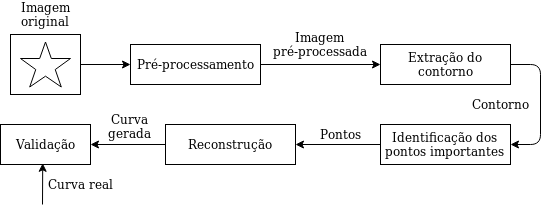
\includegraphics[width=1\textwidth]{img/diagrama.png}
        \end{center}
      \end{figure}
    
    \end{frame}
    
    \section{Pré-processamento}
    
    \begin{frame}
      \frametitle{Pré-processamento}
      \framesubtitle{Suavização}
    
        \begin{itemize}
          \item "Borrar" a imagem, eliminando alguns ruídos.
          \bigskip
          \item Utilização de filtro gaussiano, Perona-Malik ou outros.
        \end{itemize}
        
        \begin{figure}[hbt]
        \begin{center}
            \caption{Imagem original em tons de cinza e suavizada.}
            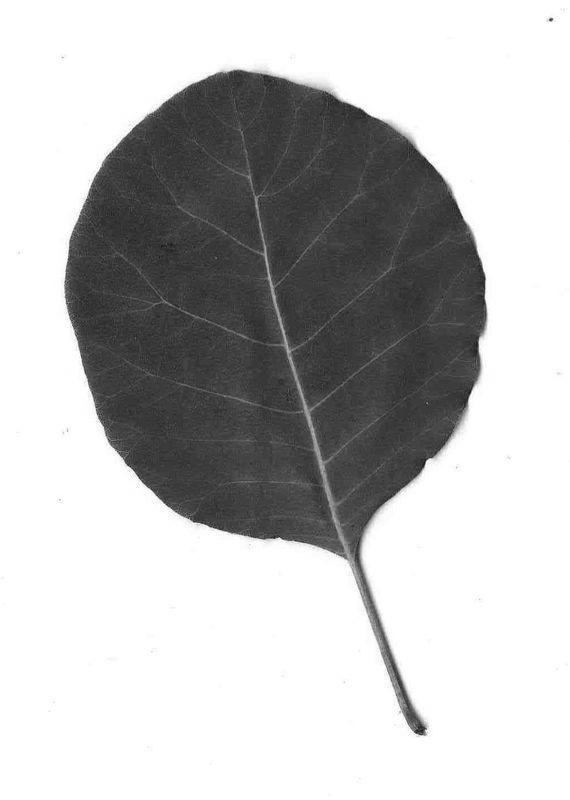
\includegraphics[width=0.3\linewidth]{img/leafs/01-gray.jpg}
            \quad
            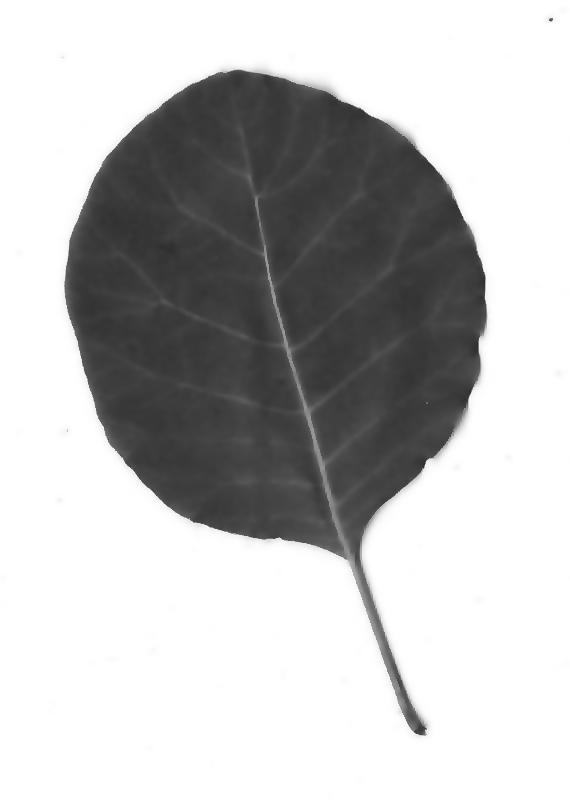
\includegraphics[width=0.3\linewidth]{img/leafs/02-smooth.jpg}
        \end{center}
        \end{figure}
    \end{frame}
    
    \begin{frame}
      \frametitle{Pré-processamento}
      \framesubtitle{Binarização}
      
        \begin{itemize}
          \item Segmentar os pixels em dois conjuntos
          \bigskip
          \item Limiarização por Otsu
        \end{itemize}
        
        \begin{figure}[hbt]
          \begin{center}
          \caption{Binarização por Otsu}
            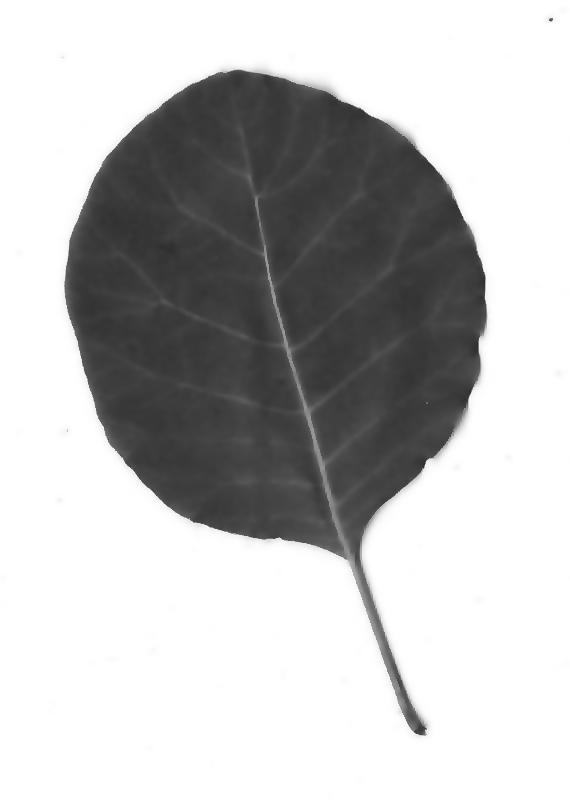
\includegraphics[width=0.3\linewidth]{img/leafs/02-smooth.jpg}
            \quad
            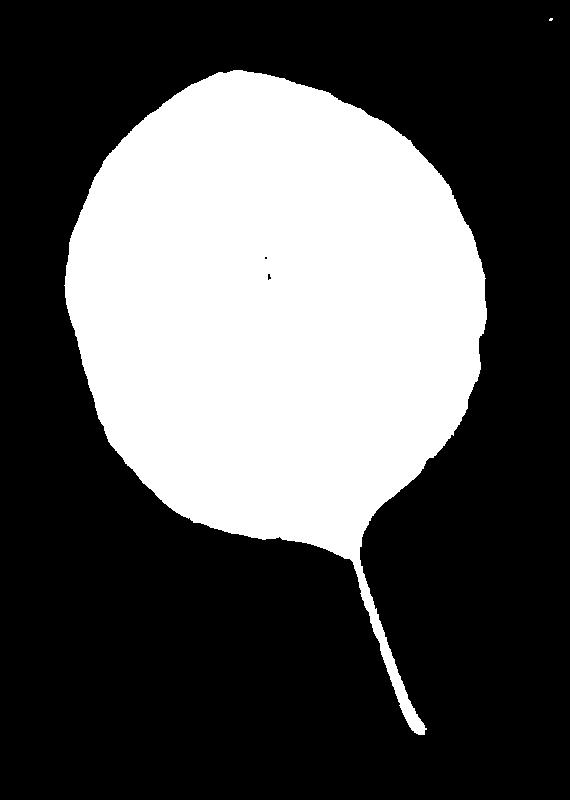
\includegraphics[width=0.3\linewidth]{img/leafs/03-otsu.jpg}
          \end{center}
        \end{figure}
    \end{frame}
    
    \begin{frame}
      \frametitle{Pré-processamento}
      \framesubtitle{Operadores Morfológicos}
      
        A partir de um conjunto de pixels $A$, elemento estruturante $B$ e valores de \textit{foreground} $z$, podemos definir: 
    
        \begin{itemize}
          \item \textbf{Erosão:} ``Diminuir" a imagem, removendo pequenas ``ilhas".
         
        \[
        A \ominus B = \{z | (B)_z \subseteq A\}
        \]

          \bigskip
          \item \textbf{Dilatação:} ``Engordar" a imagem, tapando pequenos ``buracos".
          
        \[
        A \oplus B = \{z | (\hat{B})_z \cap A \neq \emptyset\}
        \]
        \end{itemize}
    \end{frame}
    
    \begin{frame}
      \frametitle{Pré-processamento}
      \framesubtitle{Operadores Morfológicos}
    
        \begin{figure}[hbt]
          \begin{center}
          \caption{Erosão seguida de dilatação}
            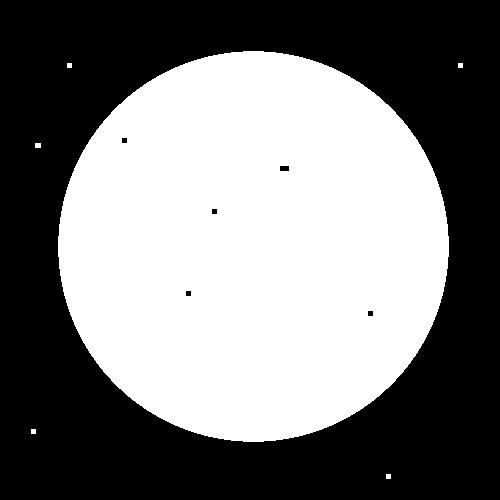
\includegraphics[width=0.3\linewidth]{img/ball/03-otsu.jpg}
            \quad
            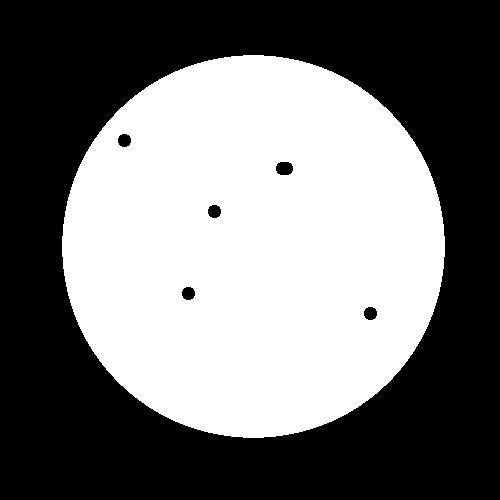
\includegraphics[width=0.3\linewidth]{img/ball/04-erode.jpg}
            \quad
            
\includegraphics[width=0.3\linewidth]{img/ball/05-dilate.jpg}
          \end{center}
        \end{figure}
        
    \end{frame}
    
    \begin{frame}
      \frametitle{Pré-processamento}
      \framesubtitle{Extração do contorno}
    
        \begin{itemize}
          \item Com a imagem já processada, fica fácil extrair o contorno.
          \item Acompanha a borda do objeto, e verifica se seus vizinhos também pertencem ao objeto.
        \end{itemize}
        
        \begin{figure}[hbt]
          \begin{center}
          \caption{Método \textit{contour following}~\cite{book_shape}}
          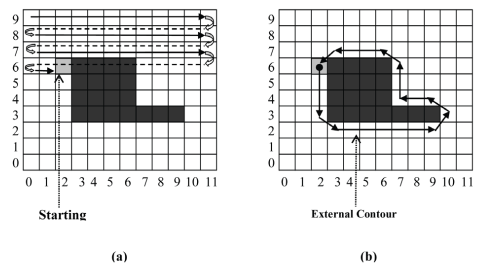
\includegraphics[width=0.6\textwidth]{img/contorno.png}
          \end{center}
        \end{figure}
    \end{frame}
    
    \begin{frame}
      \frametitle{Pré-processamento}
      \framesubtitle{Extração do contorno}
        
        \begin{figure}[hbt]
          \begin{center}
          \caption{Em \textcolor{blue}{azul}, o contorno extraído do objeto}
            
\includegraphics[width=0.35\linewidth]{img/ball/05-dilate.jpg}
            \quad
            
\includegraphics[width=0.35\linewidth]{img/ball/06-borda.png}
          \end{center}
        \end{figure}
        
    \end{frame}
    
%%%%%%%%%%%%%%%%%%%%%%%%%%%%%%%%%%%%%%%%%%%%%%%%%%%%%%%%%%%%%%%%
    \section{Curvatura}
    
    \begin{frame}
      \frametitle{Curvatura}
      \framesubtitle{Definição}
        Seja uma curva regular parametrizada por $t \rightarrow (x(t), y(t))$, em que $x(t)$ e $y(t)$ são funções de classe $C^2$. Sua curvatura é dada por:
        $$\kappa (t) = \frac{x'(t) y''(t) - y'(t) x''(t)}{(x'(t)^2 + y'(t)^2)^{3/2}}$$   
    \end{frame}
    
    \begin{frame}
      \frametitle{Curvatura}
      \framesubtitle{Discreta}
        \begin{itemize}
          \item As curvas extraídas das imagens serão um conjunto de posições dos pixels da imagem original, ordenadas de certa forma conveniente.
          \bigskip
          \item "Aproximação" pela utilização de operações vetoriais: cada posição é representada por um ponto (x, y).
          \bigskip
        %   $$\kappa (t) = \varphi_{t+1} - \varphi_{t-1} = \frac{y_{t - 1} - y_{t+1}}{x_{t - 1} - x_{t+1}},$$
        %   em que $\varphi_t$ é a direção do gradiente do pixel $t$ da curva.
        \end{itemize}
    \end{frame}
    
%%%%%%%%%%%%%%%%%%%%%%%%%%%%%%%%%%%%%%%%%%%%%%%%%%%%%%%%%%%%%%%%
    \section{Extração das características robustas}
    
    \begin{frame}
      \frametitle{Características robustas em $\mathbb{R}^2$}
      \framesubtitle{Definição}
        \begin{itemize}
          \item Pontos de inflexão e vértices (pontos extremantes).
          \bigskip
          \item Pelo teorema dos quatro vértices \cite{book_manfredo}, toda curva fechada e simples tem, pelo menos, quatro vértices.
        \end{itemize}
        % \bigskip
          \begin{figure}[hbt]
            \begin{center}
            \caption{À esquerda, 4 vértices de uma elipse~\cite{book_difgeosing} e, à direita, pontos importantes de uma curva com $\kappa(x) = x^3 - 2x$}
            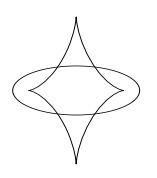
\includegraphics[width=.2\textwidth]{./img/vertex.png}
            \quad
            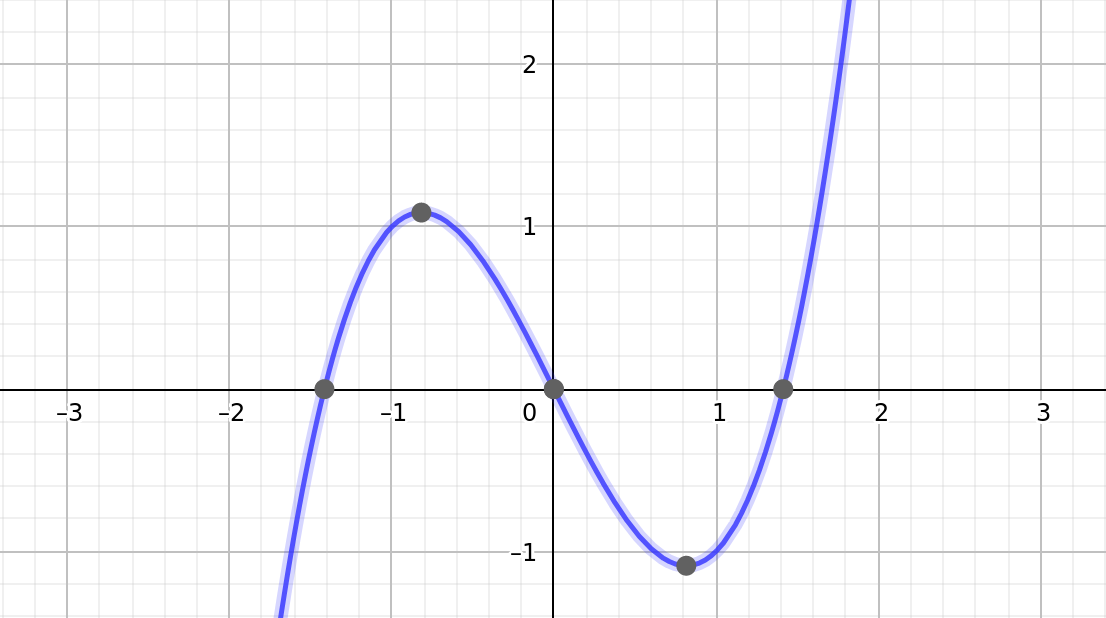
\includegraphics[width=.4\textwidth]{./img/curva.png}
            \end{center}
          \end{figure}
    \end{frame}
    
%%%%%%%%%%%%%%%%%%%%%%%%%%%%%%%%%%%%%%%%%%%%%%%%%%%%%%%%%%%%%%%%
    \section{Reconstrução de curvas}
    
    \begin{frame}
      \frametitle{Reconstrução de curvas}
    %   \framesubtitle{}
    
        \begin{itemize}
          \item Representação a partir de curvas lineares por partes.
          \bigskip
          \item Operadores de Laplace discretos.
        \end{itemize}
        
        \begin{figure}[hbt]
            \begin{center}
            \caption{Reconstrução de uma curva fechada~\cite{book_sorkine}}
            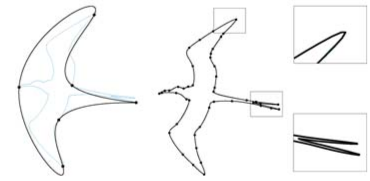
\includegraphics[width=.6\textwidth]{./img/reconstrucao.png}
            \end{center}
          \end{figure}
    \end{frame}
    
%%%%%%%%%%%%%%%%%%%%%%%%%%%%%%%%%%%%%%%%%%%%%%%%%%%%%%%%%%%%%%%%
    \section{Validação}
    
    \begin{frame}
      \frametitle{Validação}
    
        \begin{itemize}
          \item Comparação entre a curva obtida pela reconstrução e a curva original.
          \bigskip
          \item Utilização de alguma métrica de distância: quanto menor a distância, menor o erro do algoritmo.
        \end{itemize}
    \end{frame}
    
    %%%%%%%%%%%%%%%%%%%%%%%%%%%%
    \section{Referências}
    
    \begin{frame}[allowframebreaks]
      \frametitle{Referência Bibliográfica}
      \bibliographystyle{siam}
      
      \bibliography{referencias}
    \end{frame}

\end{document}
